\chapter{Sanskrit roots}

This last chapter on Sanskrit tools is about roots. We have the whole book of W.\,D.\ Whitney's Sanskrit Roots (1885) here with the full list of roots for navigation. It is a lot more convenient comparing to its printed form. The book can be opened by menu Sanskrit > {\faSix \symbol{"F4D8}} Whitney's roots.

This tool is very simple in design without the common tool bar. Its tool bar has only navigator and help. The left pane is the list of roots ordered as in the book. You can jump to a specific root by clicking an item in the list. The list can be filtered further by entering a word in the search text field. Figure \ref{fig:sanskrit-whitney} shows a root selected by the list.

\begin{figure}[!hbt]
\centering
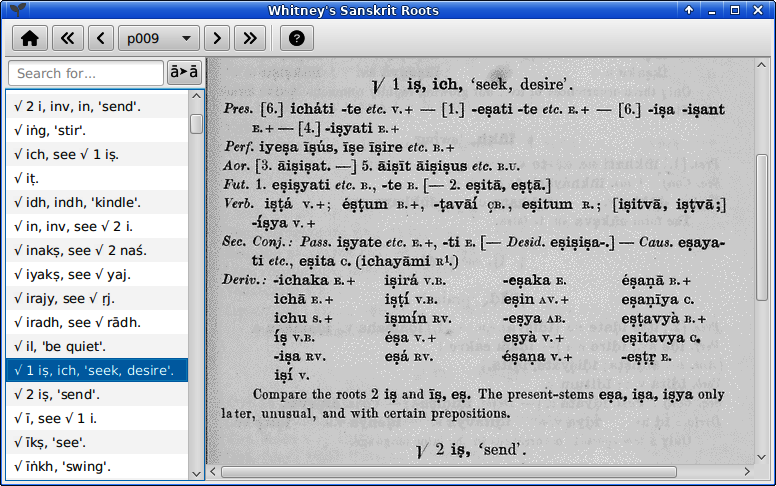
\includegraphics[width=0.9\linewidth]{images/sanskrit-whitney.png}\\
\caption{Whitney's Sanskrit roots}
\label{fig:sanskrit-whitney}
\end{figure}

Because the tool is really easy to use, I have no more words to say about it, but see the box note below for a warning.

\boxnote{Transliteration in Whitney's roots\\
Since the book was printed long time ago, it used an archaic way of encoding. Apart from accents that can be simply ignored, here are some noteworthy differences:\\
\hspace{5mm}\bullet\ \pali{\=n} is \pali{ṅ}\\
\hspace{5mm}\bullet\ \pali{ç} is \pali{ś}\\
\hspace{5mm}\bullet\ \pali{ṅ} is \pali{ṃ} (be careful)
}

Apart from this tool, we can obtain lists of roots by exploring MW dictionary as shown in Chapter \ref{chap:dict}. We have a number of grouping as described below\footnote{The information is taken from the metadata of MW dict file.} (see also Figure \ref{fig:explore-mw} on page \pageref{fig:explore-mw}).

\begin{compactitem}
\item Roots/Verbs are all entries described as roots.
\item Genuine are roots with large Devanāgarī in the print. These are around 750 entries.
\item Non-genuine are those not in the 750.
\item Westergaard are roots listed in the Westergaard Dhātupāṭha, with references to Sāyaṇa's Mādhavīya Dhātuvṛtti.
\item Whitney are roots listed by Whitney seen above, with page numbers.
\end{compactitem}

Figure \ref{fig:sanskrit-mwwhitney} shows a result of Whitney's roots, selected in an exploring mode of MW in Sanskrit dictionaries. Even though you can explore roots/verbs in other dictionaries likewise, the results in MW are most comprehensive and better organized.

\newpage
\begin{figure}[!hbt]
\centering
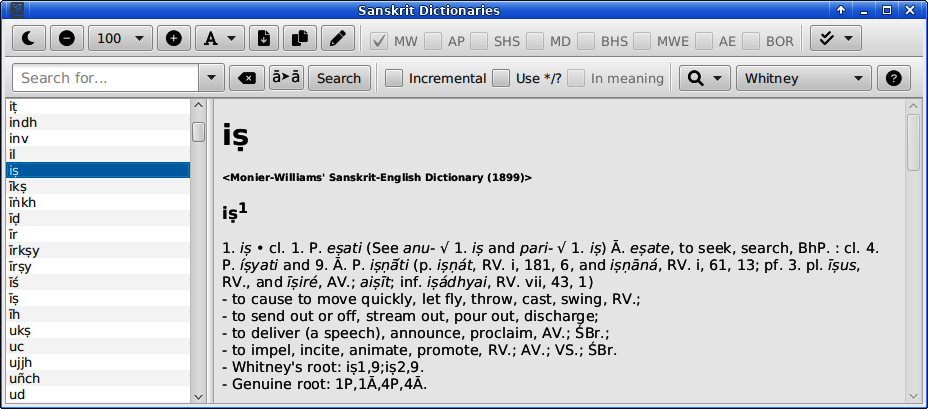
\includegraphics[width=0.9\linewidth]{images/sanskrit-mwwhitney.png}\\
\caption{Whitney's roots listed in MW dictionary}
\label{fig:sanskrit-mwwhitney}
\end{figure}

